\documentclass[12pt,letterpaper]{article}

\usepackage{amsmath, amsthm, amsfonts, amssymb}
\usepackage{microtype, parskip, graphicx}
\usepackage[comma,numbers,sort&compress]{natbib}
\usepackage{lineno}
\usepackage{longtable}
\usepackage{docmute}
\usepackage{caption, subcaption, multirow, morefloats, rotating}
\usepackage{wrapfig}
\usepackage{hyperref}

\frenchspacing

\begin{document}

\section{Model selection and adequacy}

\begin{table}[ht]
  \centering
  \begin{tabular}{rrr}
    \hline
    Model & looic \\
    \hline
    Past and vary & 12811.58 & 12807.61 \\
    No past but vary & 12834.53 & 12831.51 \\
    Past but no vary & 12836.19 & 12833.13 \\
    No past or vary & 12849.43 & 12847.08 \\
    \hline
  \end{tabular}
  \label{tab:selection}
\end{table}

% ROC model comparison
\begin{figure}[ht]
  \centering
  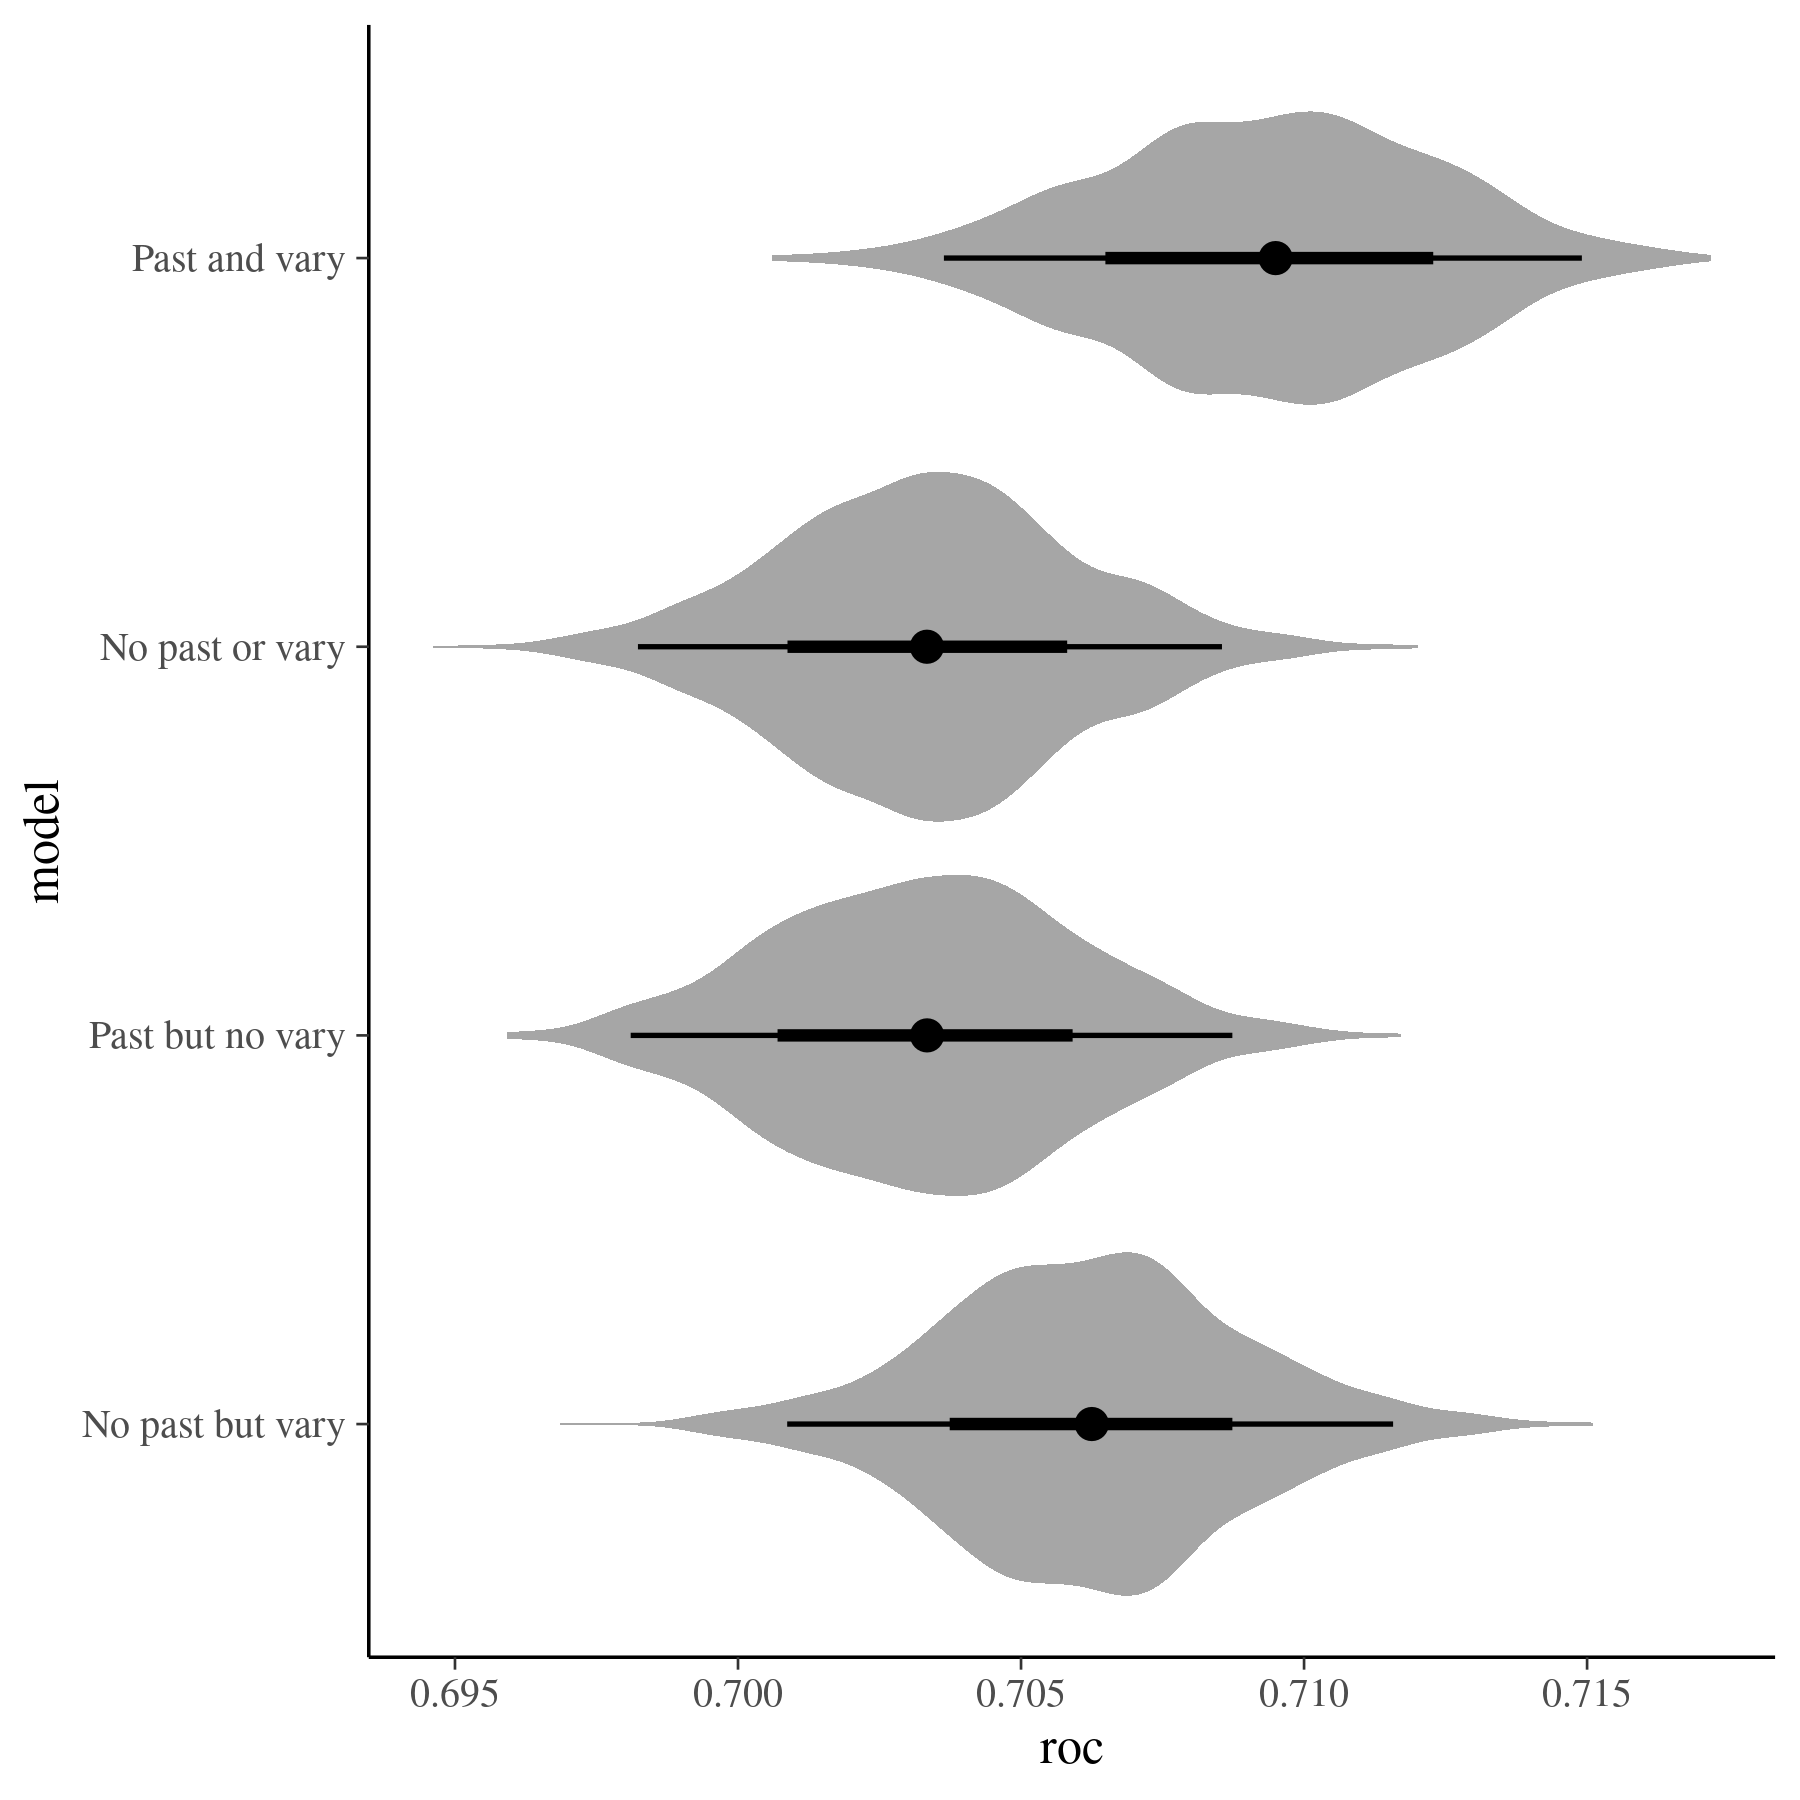
\includegraphics[width=\textwidth,height=0.5\textheight,keepaspectratio=true]{figure/roc_hist}
  \caption{Comparison of AUC estimates between the four models. These estimates are based on in-sample values. Higher values indicate greater performance.}
  \label{fig:roc_hist}
\end{figure}

% ROC model comparison time series
\begin{figure}[ht]
  \centering
  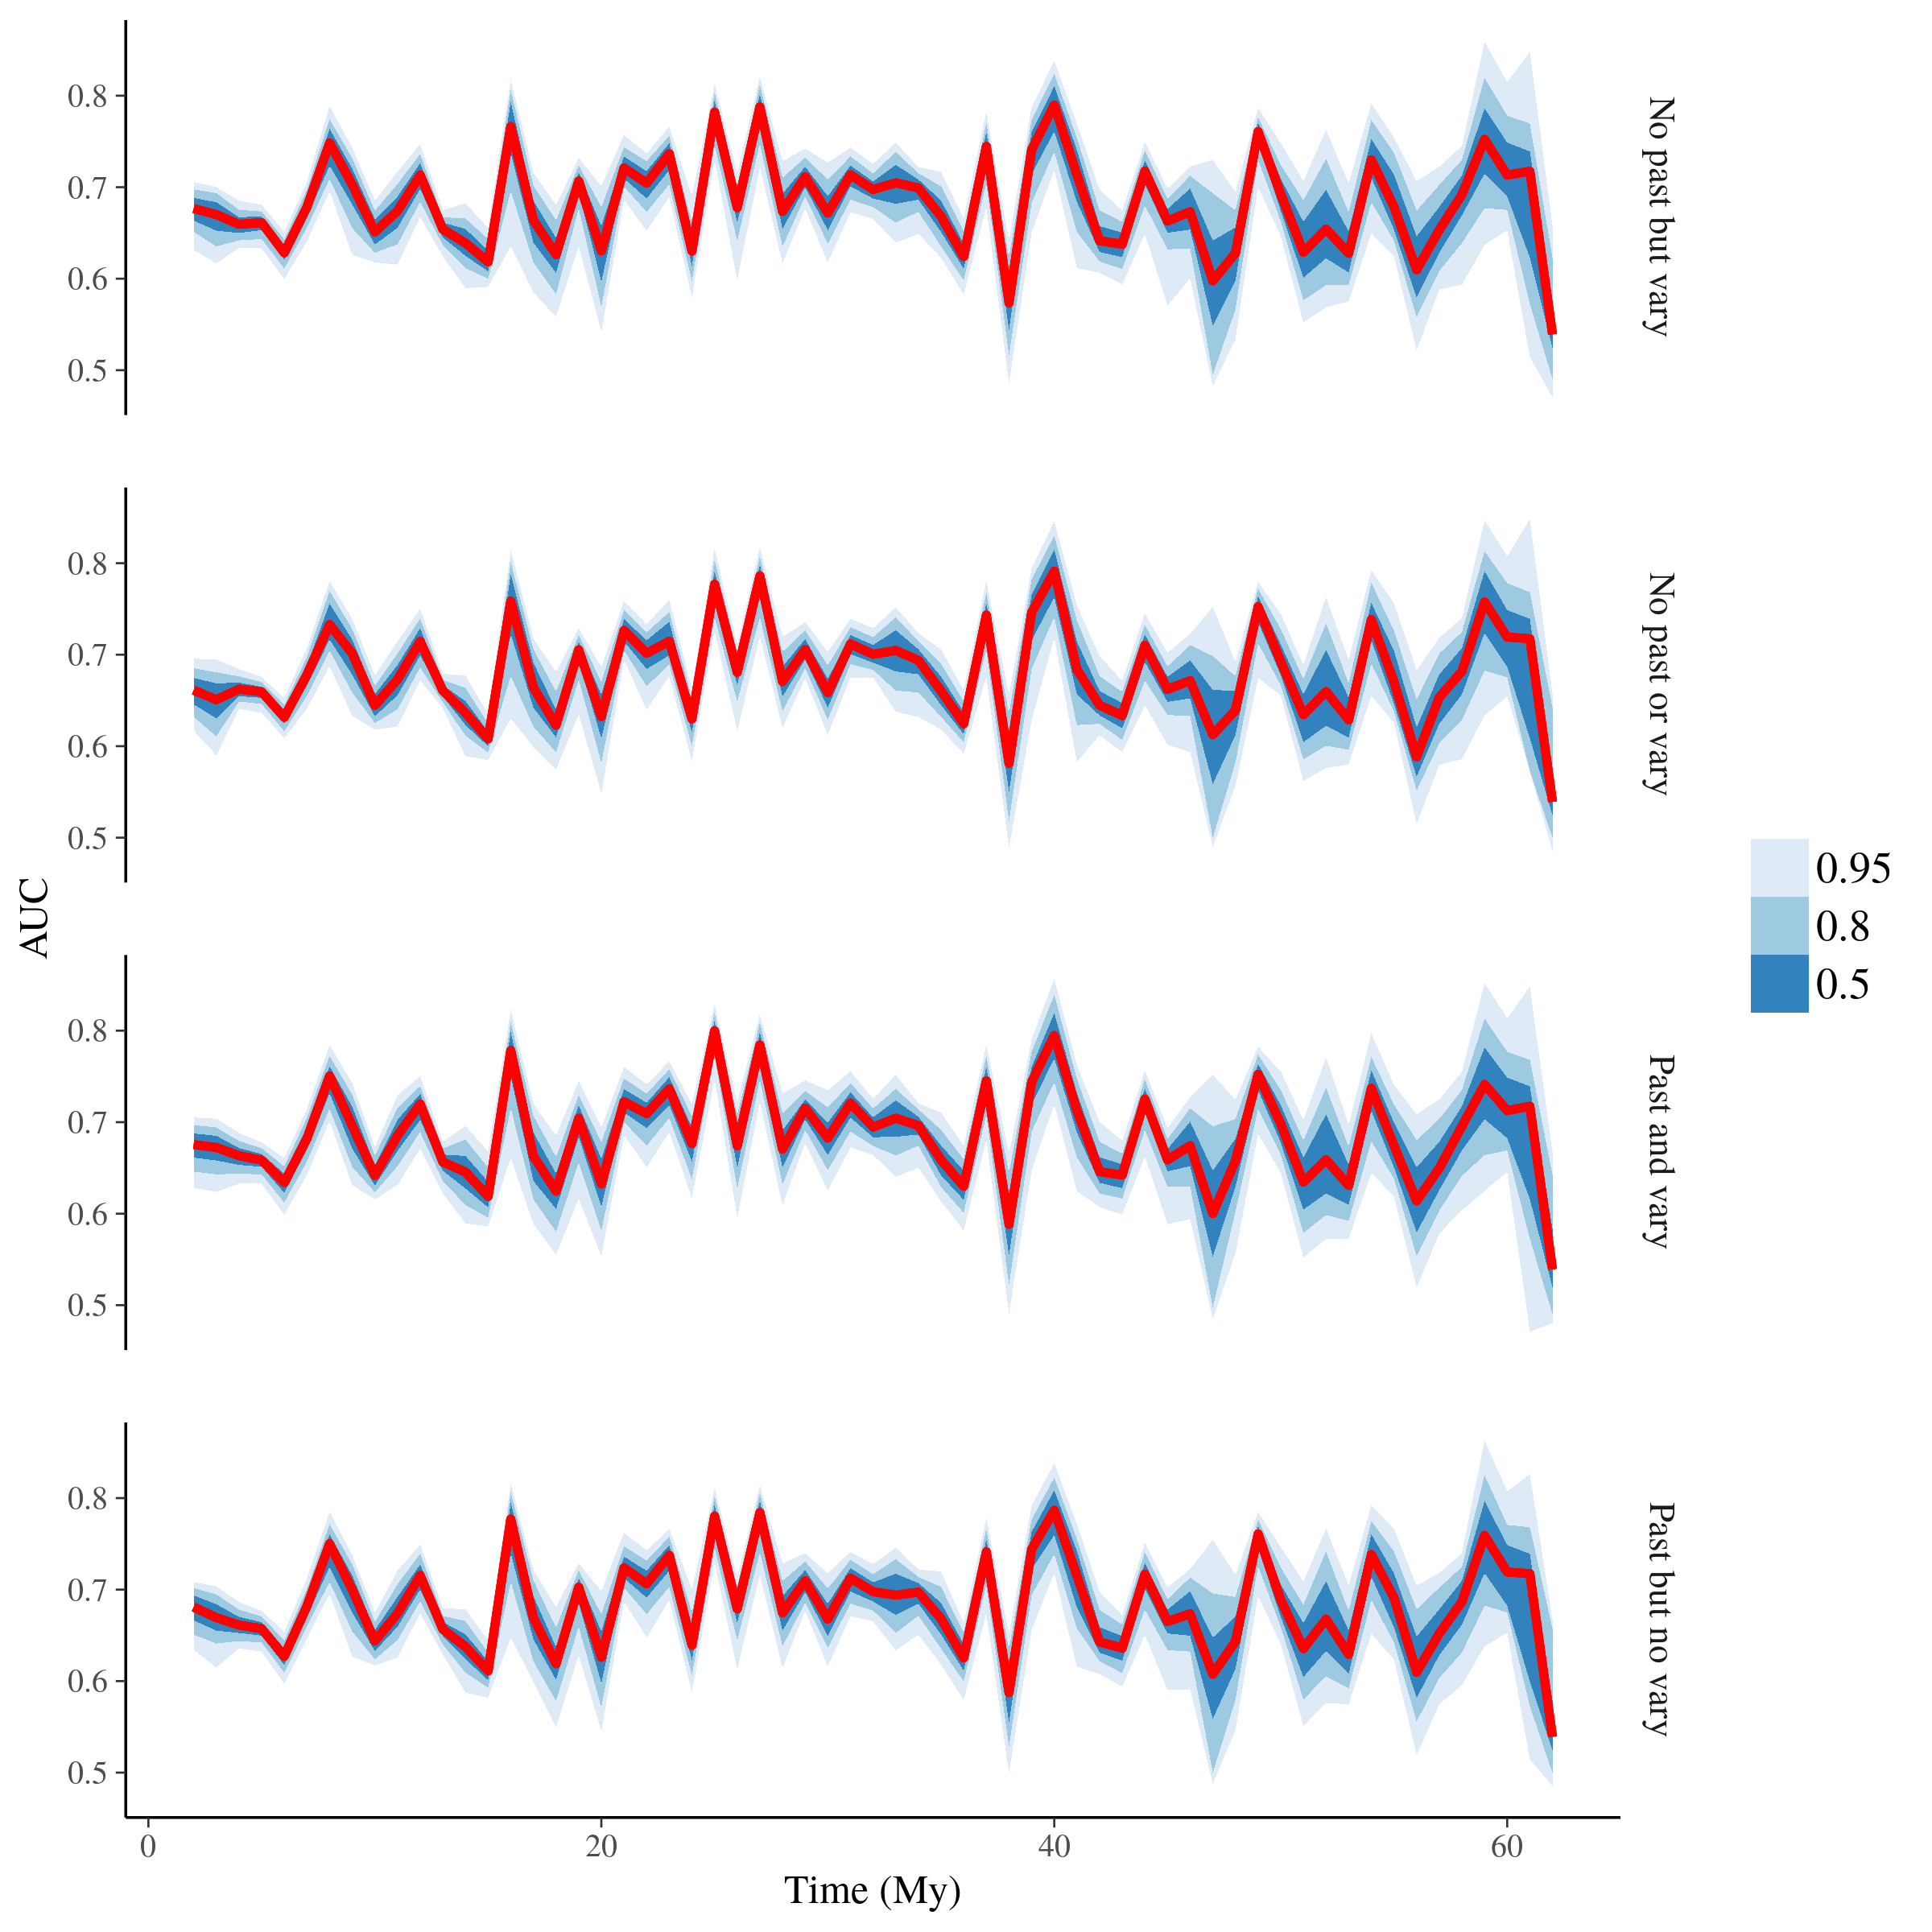
\includegraphics[width=\textwidth,height=0.5\textheight,keepaspectratio=true]{figure/roc_ts}
  \caption{Comparison of time-specific AUC values between the four models. These estimates correspond to the models ability to predict or fit that section of the data. Higher values indicate greater performance.}
  \label{fig:roc_ts}
\end{figure}


\section{Cross-validation}

% ROC OOS estimate
\begin{figure}[ht]
  \centering
  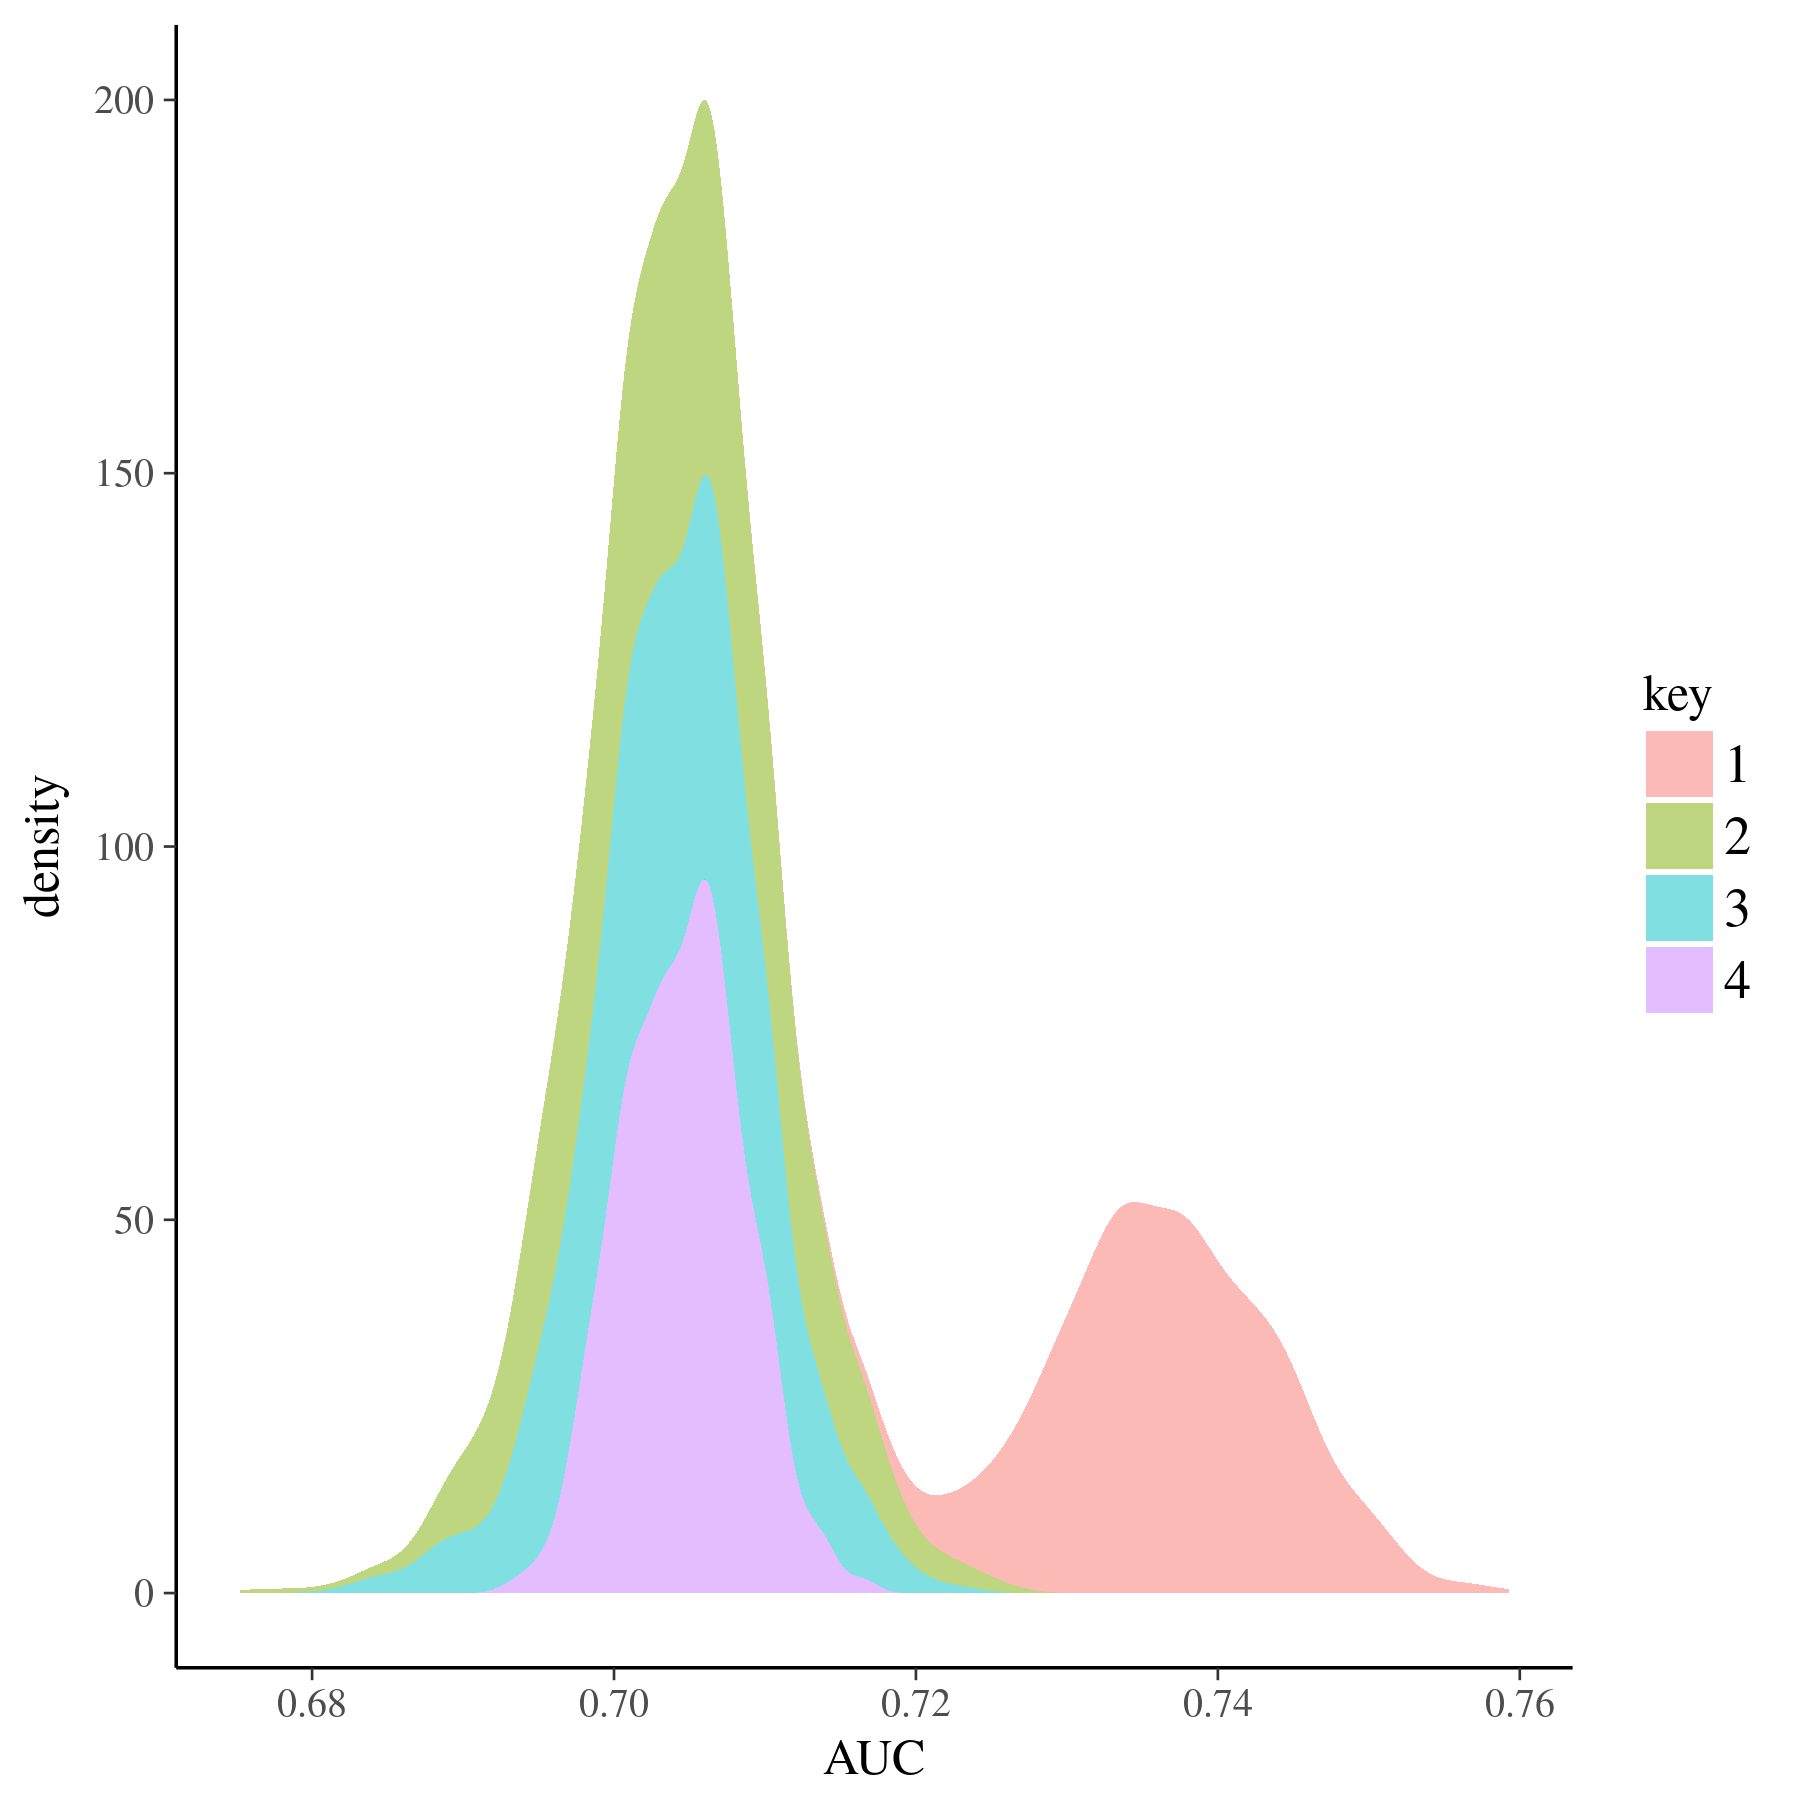
\includegraphics[width=\textwidth,height=0.5\textheight,keepaspectratio=true]{figure/fold_auc}
  \caption{Approximate out-of-sample AUC values calculated from five-fold cross-validation of the time series. The AUC estimates from each fold are labeled. Folds are numbered from oldest to youngest.}
  \label{fig:fold_auc}
\end{figure}

% ROC OOS estimate time series
\begin{figure}[ht]
  \centering
  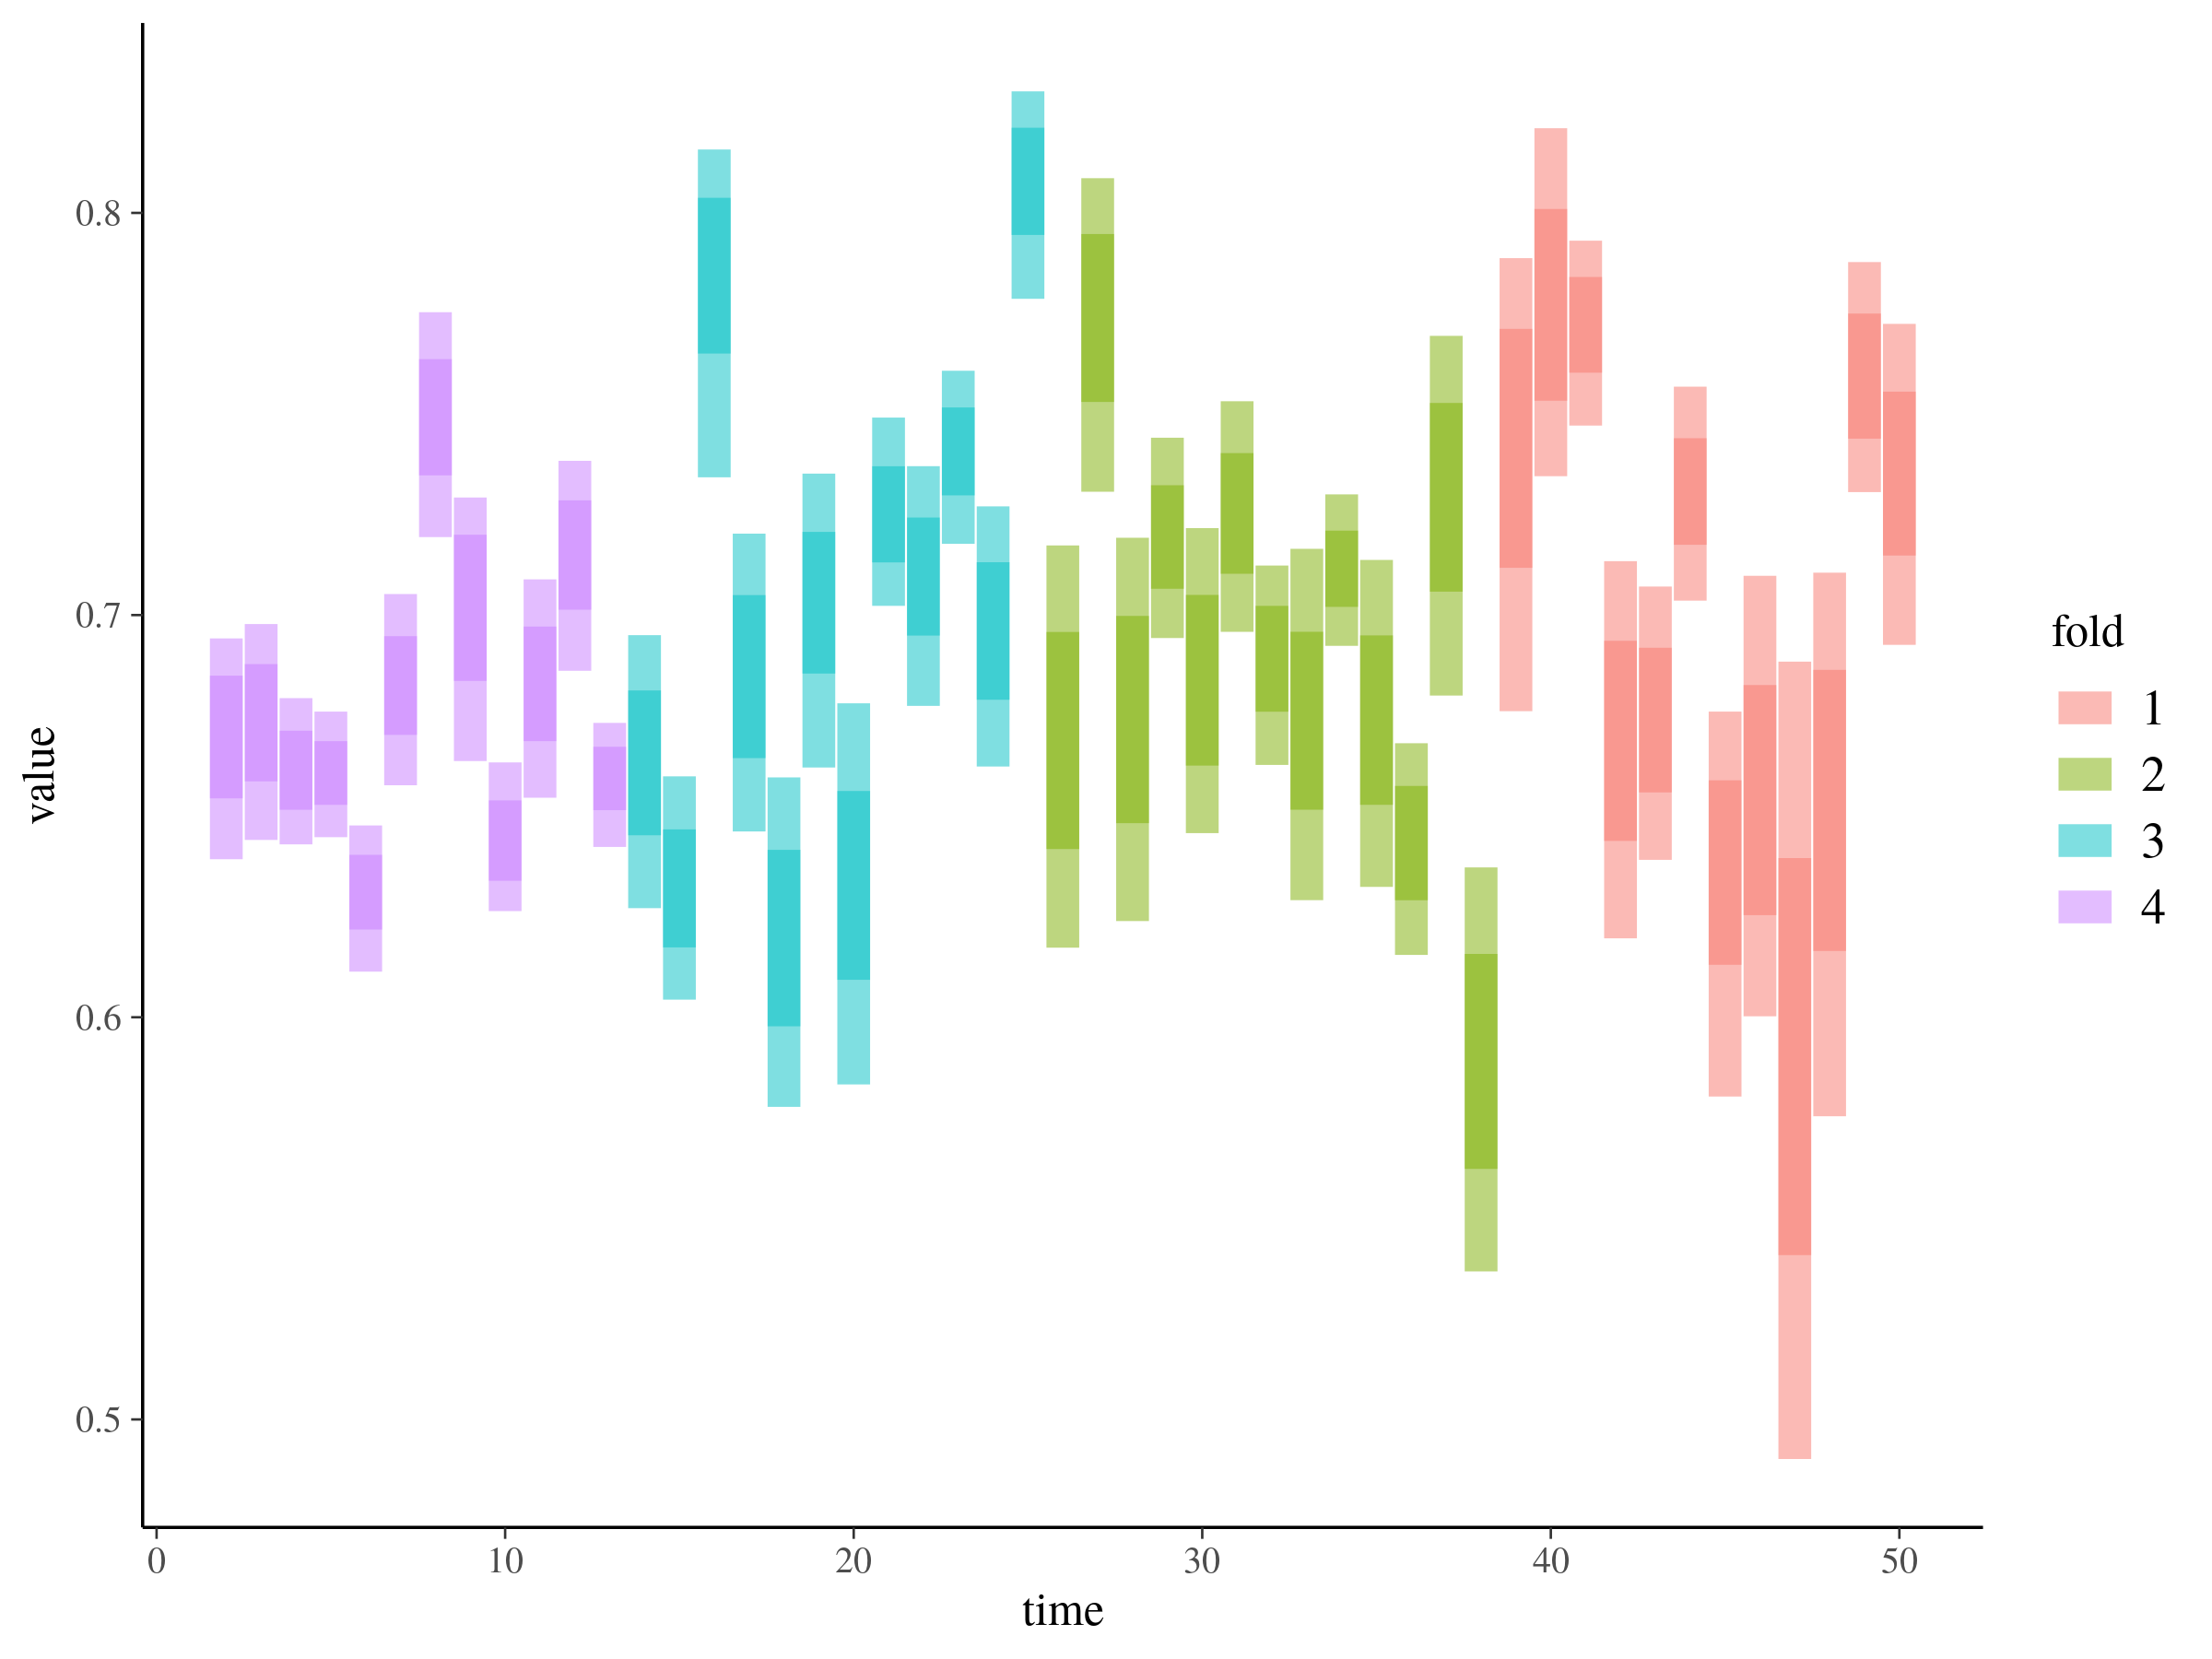
\includegraphics[width=\textwidth,height=0.5\textheight,keepaspectratio=true]{figure/fold_auc_time}
  \caption{Approximate out-of-sample AUC values calculated for each of the My intervals using five-fold cross-validation of the time series. The AUC of the individual My intervals within each fold is plotted to highlight the heterogentity in performance within and between folds. The AUC estimates from each fold are labeled and are numbered from oldest to youngest.}
  \label{fig:fold_auc_time}
\end{figure}


\section{Parameter estimates}

% effects, average
\begin{figure}[ht]
  \centering
  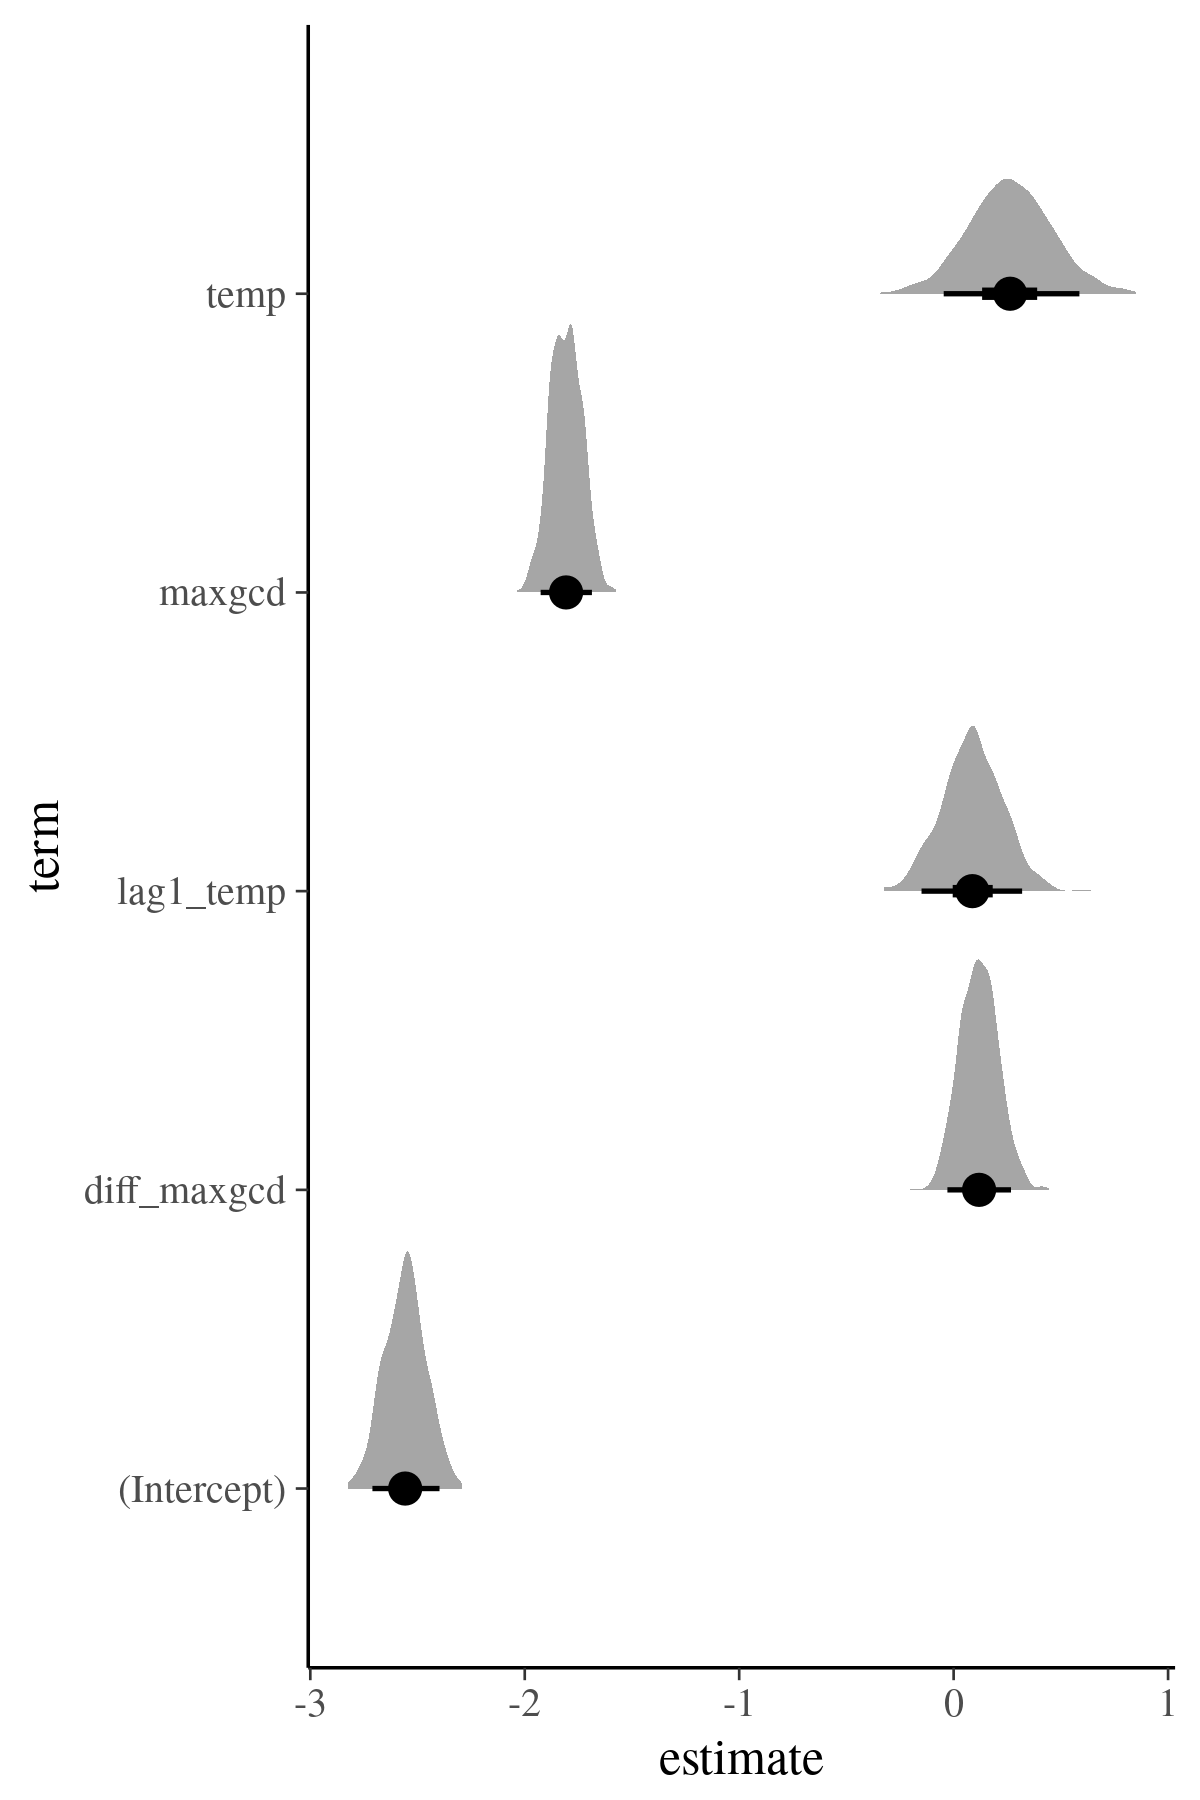
\includegraphics[width=\textwidth,height=0.5\textheight,keepaspectratio=true]{figure/effect_est}
  \caption{Estimates of the overall average covariate effects. These are averaged both over time and across phyla. The entire posterior is presented, with the median estimate labeled and 80\% credible intervals.}
  \label{fig:effect_est}
\end{figure}

% effects, time series
\begin{figure}[ht]
  \centering
  \includegraphics[width=\textwidth,height=0.5\textheight,keepaspectratio=true]{figure/effect_time_group}
  \caption{Covariate effect estimates for the effect of geographic range and the change in geographic range for all time points and phyla. The red line corresponds to the median estimate at each time, the dark blue area corresponds to the 50\% credible interval, the medium blue the 80\% credible interval, and the light-blue the 95\% credible interval.}
  \label{fig:<+label+>}
\end{figure}<++>

% variance components

% risk estimate compared to change in geo-range


\end{document}
